\section{Physikalisches Modell}
\label{sec:Physikalisches Modell}

% Welche Formeln sollten gültig sein?
%     \item Wie könnte das System modelliert werden?
%     \item Welche möglichen Störgrößen würden Sie erwarten?
% Was für ein System wollen Sie betrachten, was für Gesetzmäßigkeiten liegen vor?

Die verwendeten Spulenkörper sind geometrisch allesamt Zylinder. Somit ist für die Modellierung der Drahtwicklung nur die Umrandungskurve der Grundfläche und die Höhe des Zylinders ausschlaggebend. Der gewickelte Draht kann dementsprechend als Raumkurve aufgefasst werden, woraus wiederum das Verhältnis der Winkelgeschwindigkeit $\omega$ von Hauptachse $HA$ und Nebenachse $NA$ abgeleitet werden kann. Für eine parallele Wicklung besteht ein linearer Zusammenhang zwischen den Winkelgeschwindigkeiten der Achsen. Es gilt:

\begin{equation}
    \omega_{HA} = \pm K_{xy} \cdot \omega_{NA}
\end{equation}
Das Vorzeichen bestimmt hier die Wicklungsrichtung der jeweiligen lage. Für den Skalierungsfaktor $K_{xy}$ gilt der folgende Zusammenhang:

\begin{equation}
    \label{eq:achsenskalierungsfaktor}
    K_{xy_{ideal}} = \frac{h_G}{D \cdot 2\pi} 
\end{equation}
wobei $D$ den Drahtdurchmesser in \si{\milli\metre} und $h_G$ die Ganghöhe, bzw. Steigung, der Trapezspindel in \si{\milli\metre\per 2\pi} beschreibt. Abweichungen vom idealen Skalierungsfaktor können aufgrund von mehreren Störgrößen auftreten. Hierunter fallen das Umkehrspiel der Trapezmutter, Stepverluste der Motoren, elastische Verformung der Konstruktion und die Änderung des Drahtaustrittswinkels durch Verlaufen des Drahtes, bedingt durch Reibung zwischen Spulenkörper und Wickelmedium, oder Draht auf Draht. Da es für uns mit dem vorhanden Setup nicht möglich war die Störgrößen zu isolieren und einzeln zu vermessen, werden diese in dem Korrekturfaktor $C$ zusammengefasst. Daraus folgt für den realen Achsenskalierungsfaktor der folgende Zusammenhang:

\begin{equation}
    \label{eq:achsenskalierungsfaktor_real}
    K_{xy} = \frac{h_G}{D \cdot 2\pi} \cdot C
\end{equation}
Hieraus abgeleitet ergibt sich für, hardware bedingt, das Stellkonzept, dass immer der, sich schneller zu drehende, Motor angesteuert wird und der zweite Motor diesem immer, skaliert mit $K_{xy}$, folgt. \newline \newline



% Drahtspannung aka Spannsystem
Bedingt durch die Konstruktion des Spannsystems (siehe \autoref{sec:Mechanik}) ergeben sich mehrere auf den Draht wirkende Kräfte, welche in \autoref{fig:spannsystem_kraefte} eingezeichnet sind.
% #TODO:graphic ändern
\begin{figure}[H]
    \centering
    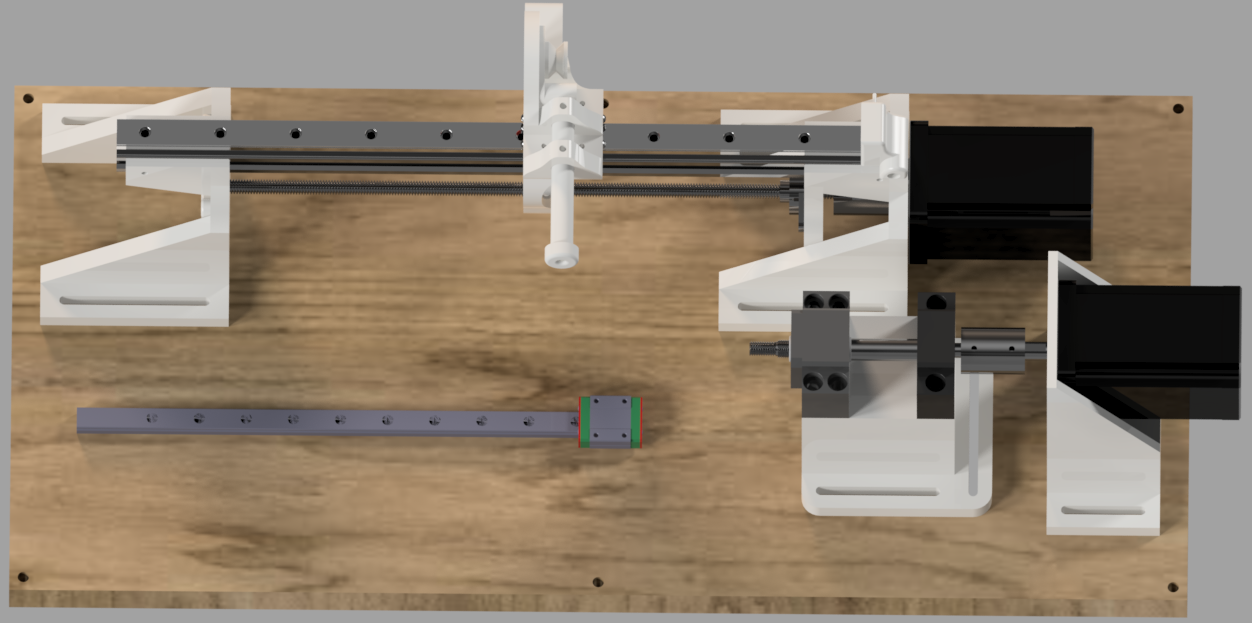
\includegraphics[width=0.25\textwidth]{./winder_render.png}
    \caption{a nice plot}
    \label{fig:spannsystem_kraefte}
\end{figure}
Die rücktreibende Kraft $F_R$, welche durch den Anpressdruck der Filzflächen entsteht, wird, während des Wickelprozesses, als annähernd konstant angenommen, da nur Gleitreibung vorliegt. Währen der Startphasen wurde eine kurzzeitig erhöhte Drahtspannungskraft erwartet, da zuerst die vorliegende Haftreibung überwunden werden muss. Durch die in \autoref{sec:Mechanik} getroffenen Annahmen muss für die Kraft am Wägezellenkugellager

\begin{equation}
    \label{eq:wz_kraft}
    F_{WZ} = 2  \tau = 2  F_T
\end{equation}
gelten, wobei $\tau$ die Drahtspannungskraft beschreibt. Unter der Annahme, dass die Positionierung des Dancerarmes über der Wickelmaschine so erfolgt, dass der Winkel von einlaufenden und auslaufendem Draht 180° einschließt, gilt für die Federkraft $F_F$, mit der Federkonstante $k$, in Ruheposition:

\begin{equation}
    F_F = 2 \cdot k  \cdot F_T
\end{equation}
Die Auslenkung der Feder wird idealisiert immer als vertikal angenommen. Für eine konstante Tangentialgeschwindigkeit $v$ an der Spulenkörperoberfläche gilt für die Spulenkraft $F_{SP}$

\begin{equation}
    F_{SP} = -F_T
\end{equation}
, bzw.

\begin{equation}
    0 \overset{!}{=}  F_{SP} + F_R
\end{equation}
Die Änderung der Drahtgeschwindigkeit bei der Wickelung mehrerer Lagen wurde aufgrund der geringen Dicke des Drahtes und der geringen Anzahl an geschichteten Lagen im Experiment ebenfalls vernachlässigt.
Beim Wickeln eines rotationssymetrieschen Spulenkörpers wäre die Drahtspannung ohne Dancerarm theoretisch am Anfang etwas höher, da aufgrund der Haftreibung $F_R$ größer ist, und danach konstant. Durch diesen Spannungsunterschied beim Start des Systems ändert sich, bei eingebautem Dancerarm, die Auslenkung der Feder des Arms und wegen der Trägheit des Systems schwingt dieses um die neue Ruheposition. Im theoretisch ideal Fall würde diese Schwingung mit der Zeit abklingen, in einer realen Anwendung ist dies aber nicht zu erwarte, da das gesammte System nie perfekt starr ist und selbst auch immer Schwingt, was zu unterschiedlichsten Überlagerungen führen kann.\newline
Für Spulenkörper mit quadratischer, oder rechteckiger Grundfläche ergibt sich keine gleichmäßige Drahtgeschwindigkeit, da abhängig vom bewegten Winkel unterschiedlich viel Draht eingezogen wird. Somit ist auch die Drahtspannung, ohne Dancerarm, nicht konstant. Wird der Dancerarm verwendet, so ändert sich die Position des Arms bei jeder Spannungsänderung, wobei es, wie bereits weiter Oben beschrieben, zu einer Schwingung um die neue Ruheposition kommt. Da die Spannungsänderungen kontinuierlich und periodisch sind, ist hier eine erzwungene Schwingung zu beobachten.\newline

Wie sich experimentell allerdings herausstellte, weißt die Drahtspannungskraft eine Geschwindigkeitsabhängigkeit auf. Bei höherer Aufwickelgeschwindigkeit liegt auch eine höhere Drahtspannung vor. Dies lässt widerspricht dem oben beschrieben Modell und deutet auf eine geschwindigkeitsabhängige Rückstellkraft $F_{R}(v)$ hin, auf welche näher in \autoref{sec:Conclusio} eingegangen wird.










